
\subsubsection{5.1 Task Compression Clusters Exist (H-E1)}

Gap statistic analysis reveals three distinct compression response clusters. The gap criterion is satisfied: Gap(3) = 0.957 >= Gap(4) - SE(4) = 1.018 - 0.120 = 0.898.

\textbf{Table 1: Gap Statistic Results}

\begin{table}[htbp]
\centering
\resizebox{\columnwidth}{!}{%
\begin{tabular}{lll}
\toprule
k & Gap Value & Standard Error \\
\midrule
1 & -0.078 & 0.099 \\
2 & 0.713 & 0.101 \\
3 & 0.957 & 0.119 \\
4 & 1.018 & 0.120 \\
5 & 1.044 & 0.132 \\
6 & 1.003 & 0.127 \\
\bottomrule
\end{tabular}
}
\end{table}

The three clusters contain the following tasks:

\begin{itemize}
\item \textbf{Cluster 0} (6 tasks): hotpotqa, 2wikimqa, musique, dureader, lcc, repobench-p
\item \textbf{Cluster 1} (7 tasks): narrativeqa, qasper, multifieldqa\_zh, trec, triviaqa, samsum, lsht
\item \textbf{Cluster 2} (8 tasks): multifieldqa\_en, gov\_report, qmsum, multi\_news, vcsum, passage\_retrieval\_en, passage\_count, passage\_retrieval\_zh
\end{itemize}

Cluster 0 comprises multi-document QA and code tasks exhibiting high eviction sensitivity. Cluster 1 contains single-document QA and few-shot tasks with moderate sensitivity. Cluster 2 includes summarization and synthetic tasks with different compression profiles.

Silhouette score is 0.411, below the 0.5 target but indicating reasonable cluster separation.

\begin{figure}[htbp]
\centering
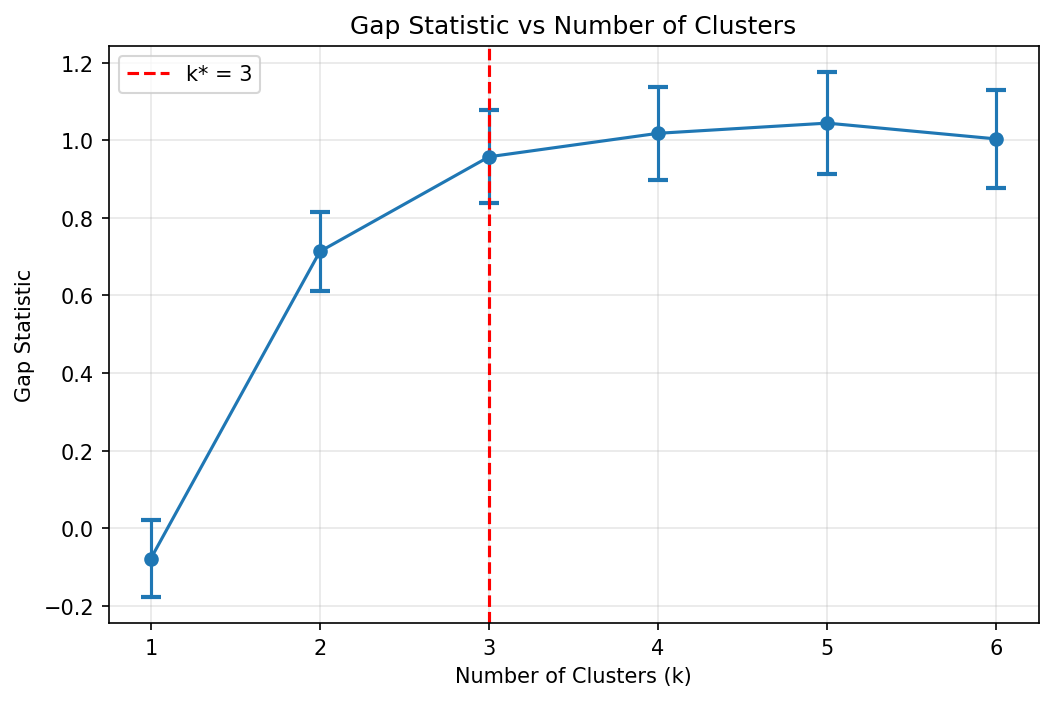
\includegraphics[width=\columnwidth]{figures/gap_curve.png}
\caption{Gap statistic curve showing k*=3}
\label{fig:gap_curve}
\end{figure}

\begin{figure}[htbp]
\centering
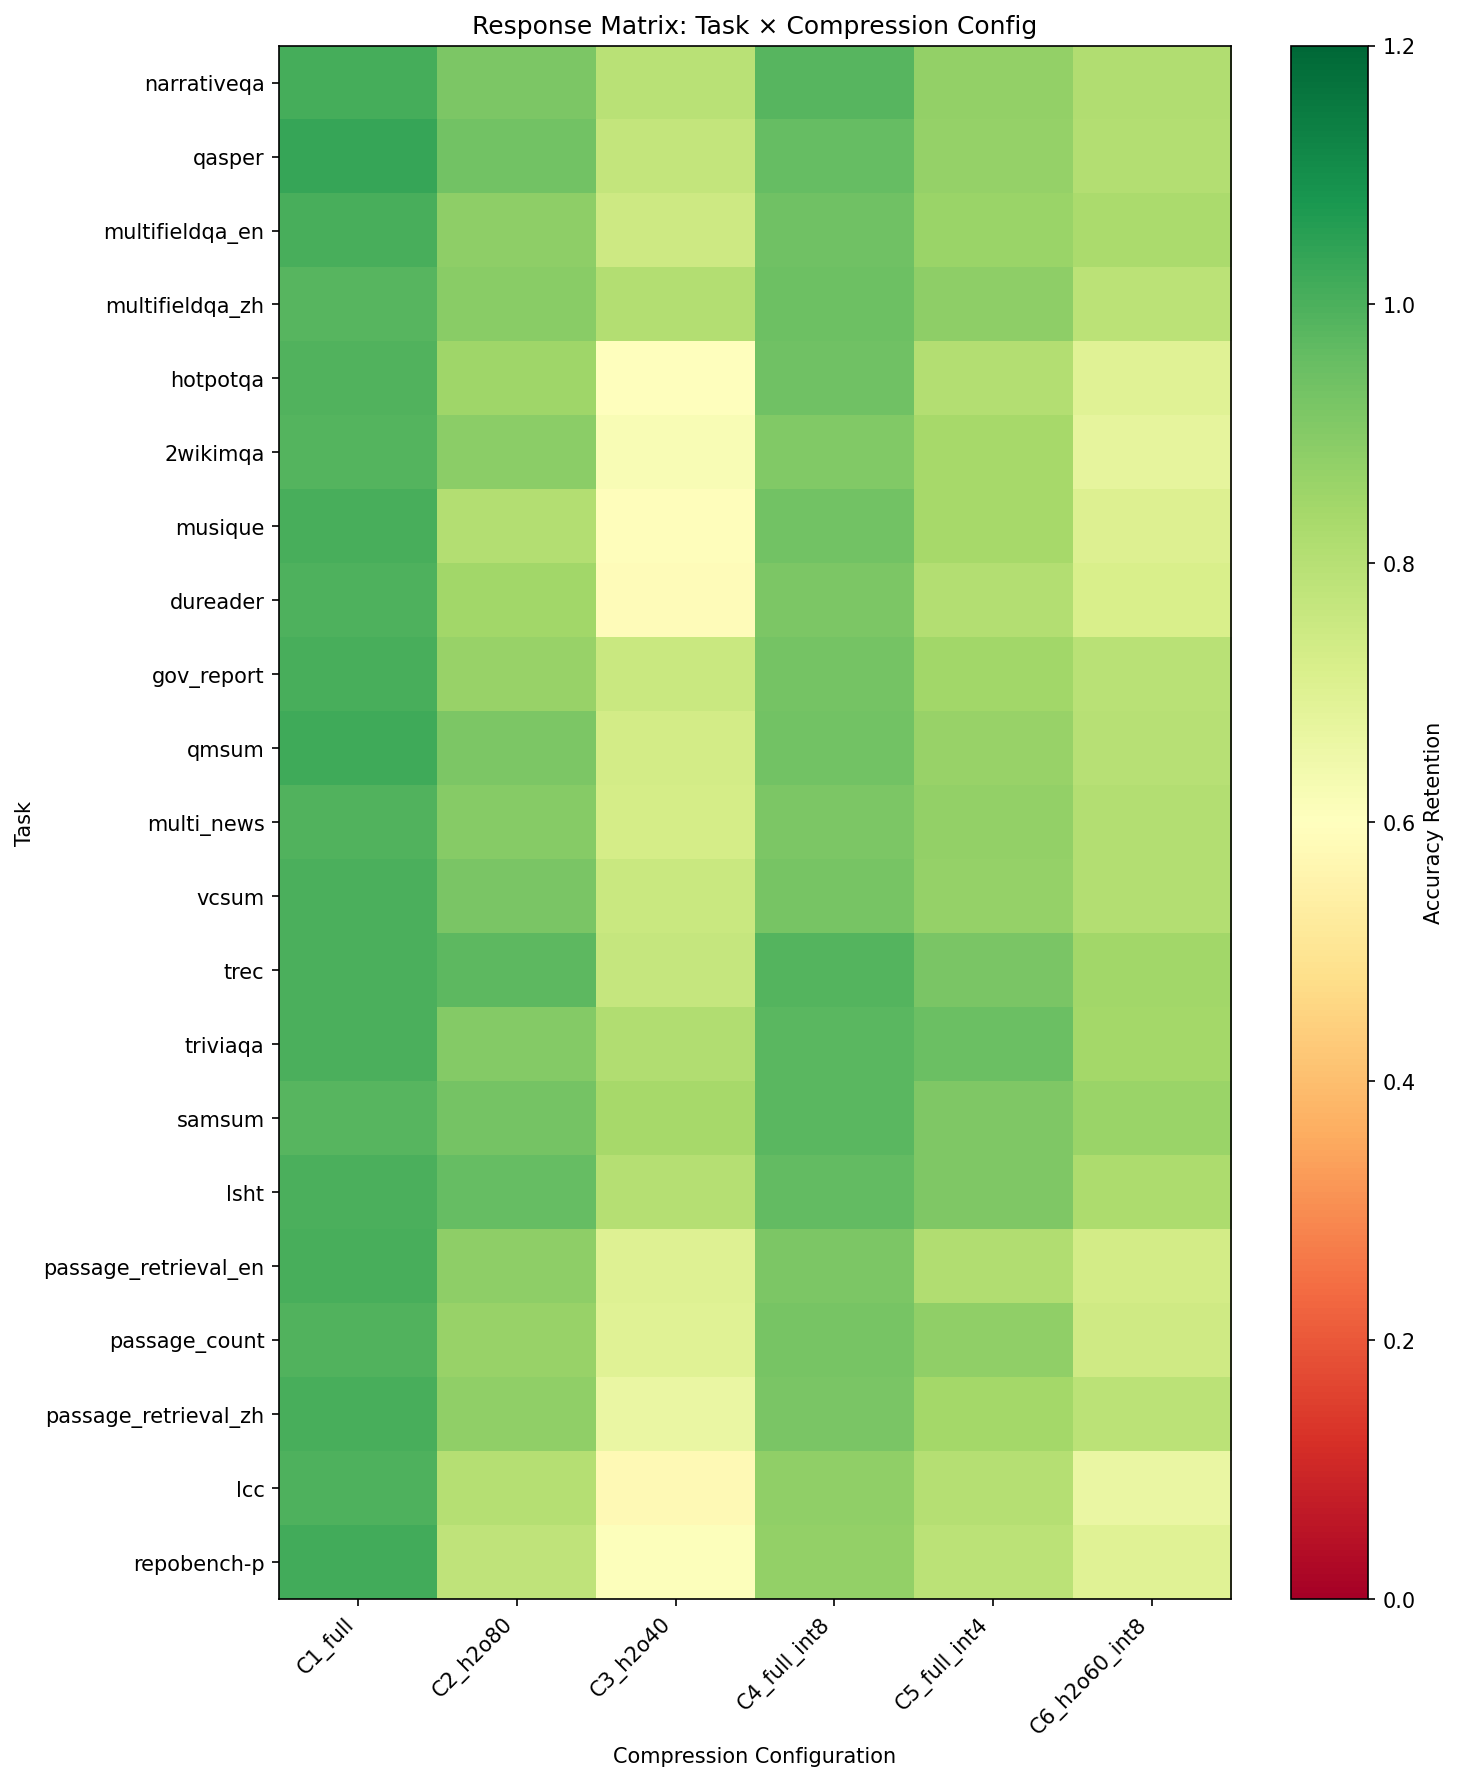
\includegraphics[width=\columnwidth]{figures/response_heatmap.png}
\caption{Task-compression response heatmap}
\label{fig:response_heatmap}
\end{figure}

\begin{figure}[htbp]
\centering
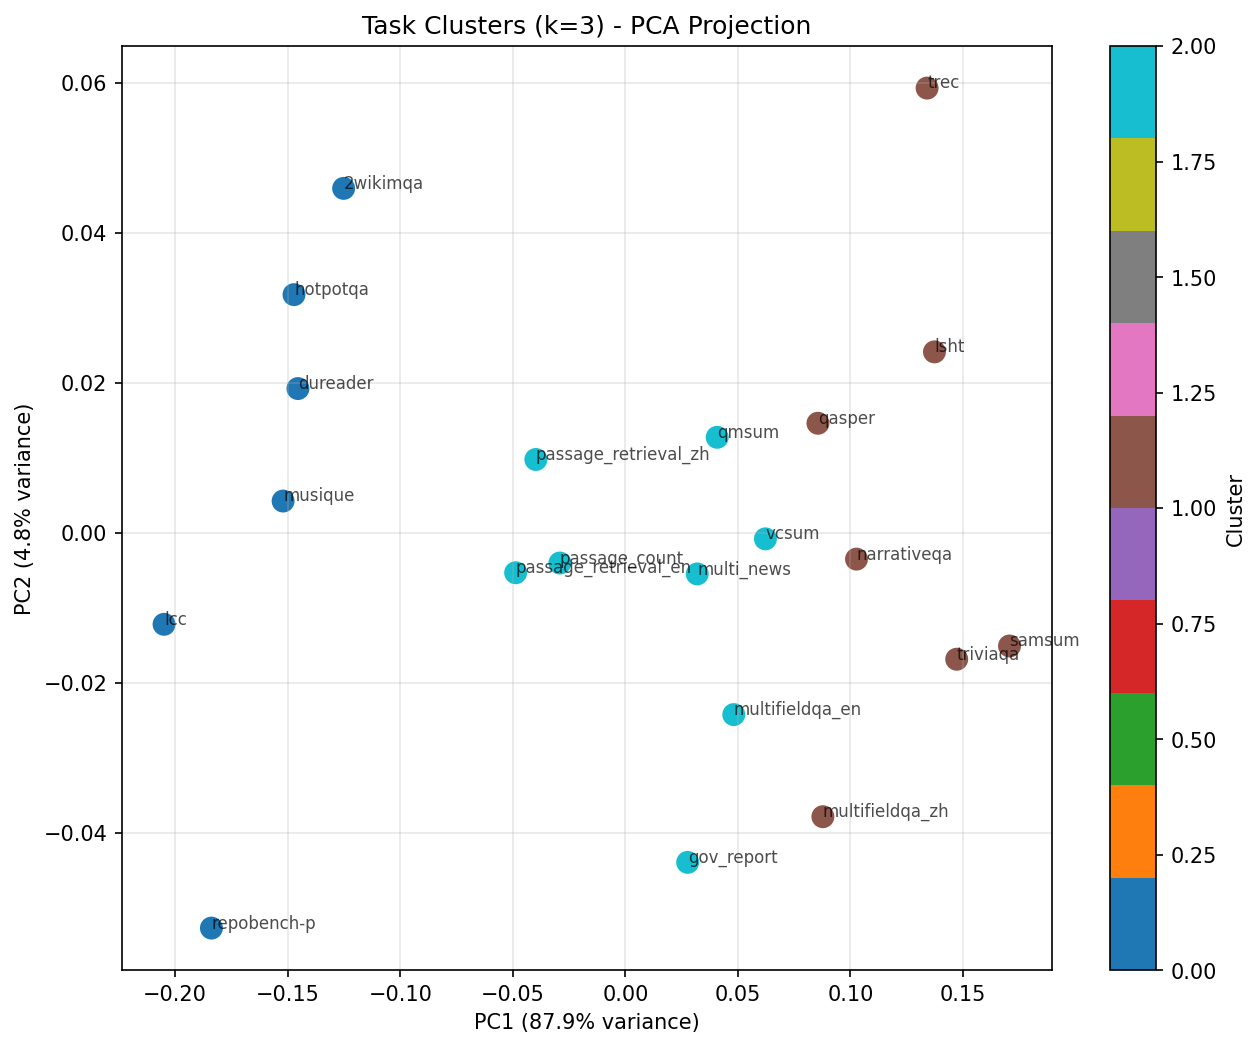
\includegraphics[width=\columnwidth]{figures/cluster_pca.png}
\caption{PCA visualization of 3 clusters}
\label{fig:cluster_pca}
\end{figure}

\subsubsection{5.2 Attention Entropy Discriminates Task Domains (H-M1)}

One-way ANOVA reveals highly significant entropy differences across the 6 LongBench domains:

\begin{table}[htbp]
\centering
\resizebox{\columnwidth}{!}{%
\begin{tabular}{ll}
\toprule
Metric & Value \\
\midrule
F-statistic & 38.05 \\
p-value & 2.92 $\times 10^{-26}$ \\
Effect size ($\eta^{2})$ & 0.522 \\
Degrees of freedom & (5, 174) \\
\bottomrule
\end{tabular}
}
\end{table}

The effect size $\eta^2$ = 0.522 indicates that 52\% of entropy variance is explained by task domain, a large effect by conventional standards.

\textbf{Table 2: Mean Entropy by Domain}

\begin{table}[htbp]
\centering
\resizebox{\columnwidth}{!}{%
\begin{tabular}{ll}
\toprule
Domain & Mean Entropy \\
\midrule
Long-dialogue History Understanding & 1.511 \\
Single-Document QA & 1.437 \\
Multi-Document QA & 1.414 \\
Code Repository Understanding & 1.408 \\
Long In-context Learning & 1.406 \\
Long Structured Data Understanding & 1.168 \\
\bottomrule
\end{tabular}
}
\end{table}

\begin{figure}[htbp]
\centering
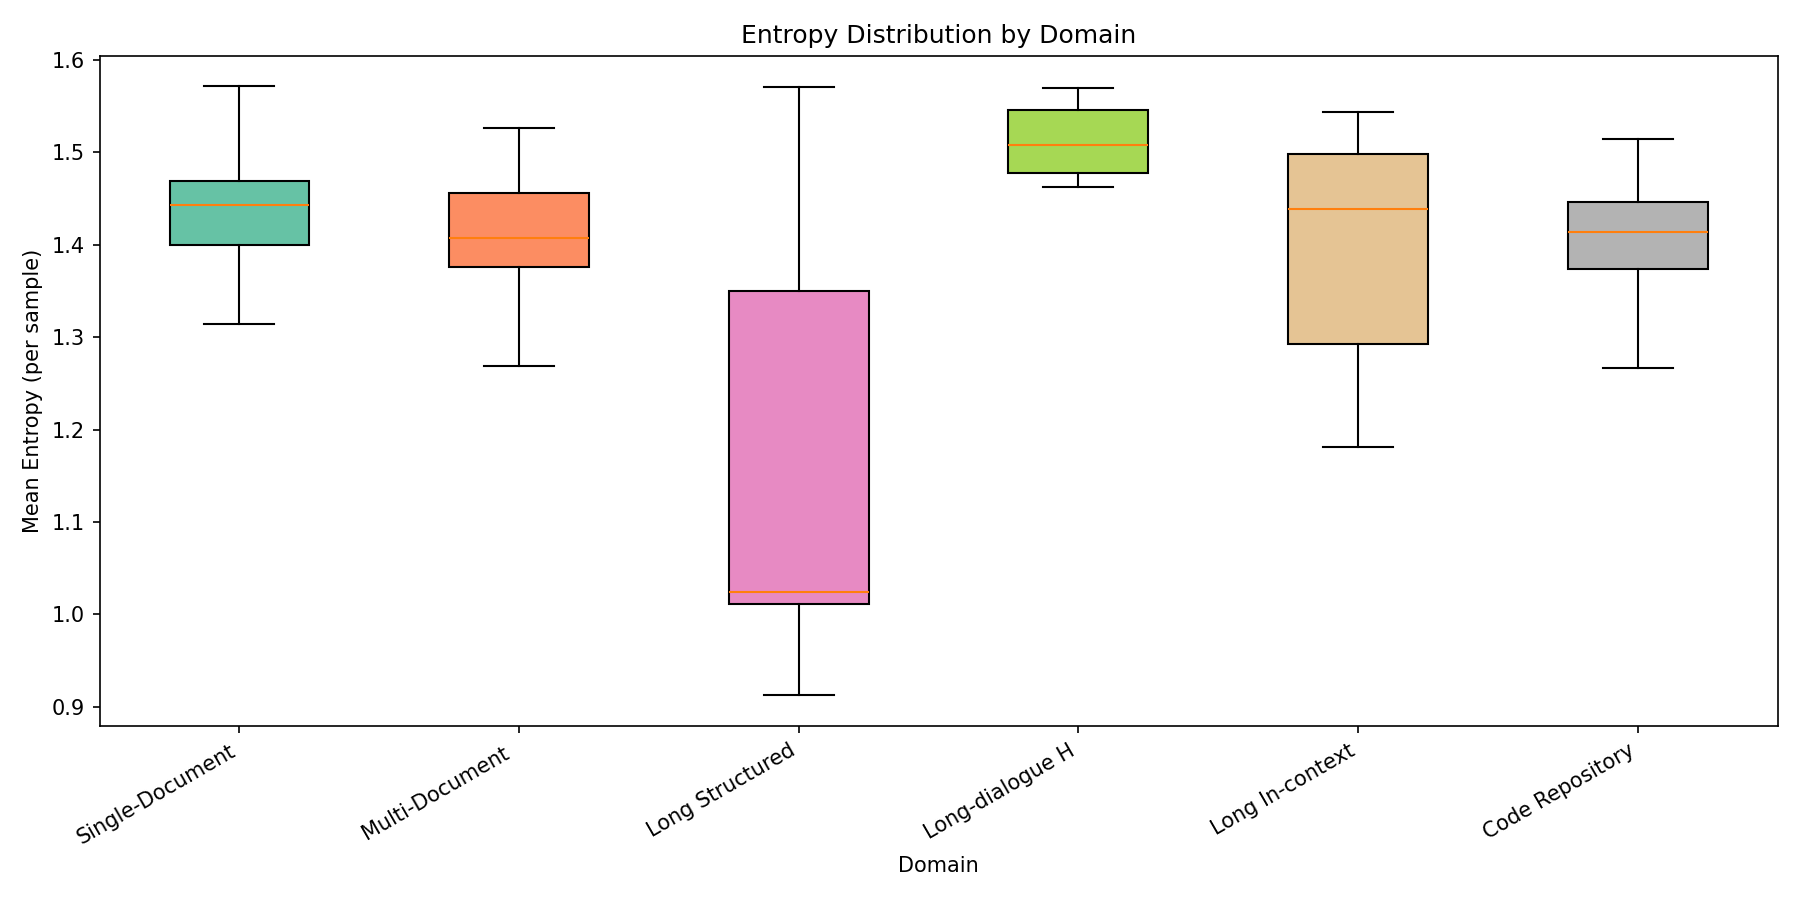
\includegraphics[width=\columnwidth]{figures/domain_boxplot.png}
\caption{Entropy distribution by task domain}
\label{fig:domain_boxplot}
\end{figure}

\begin{figure}[htbp]
\centering
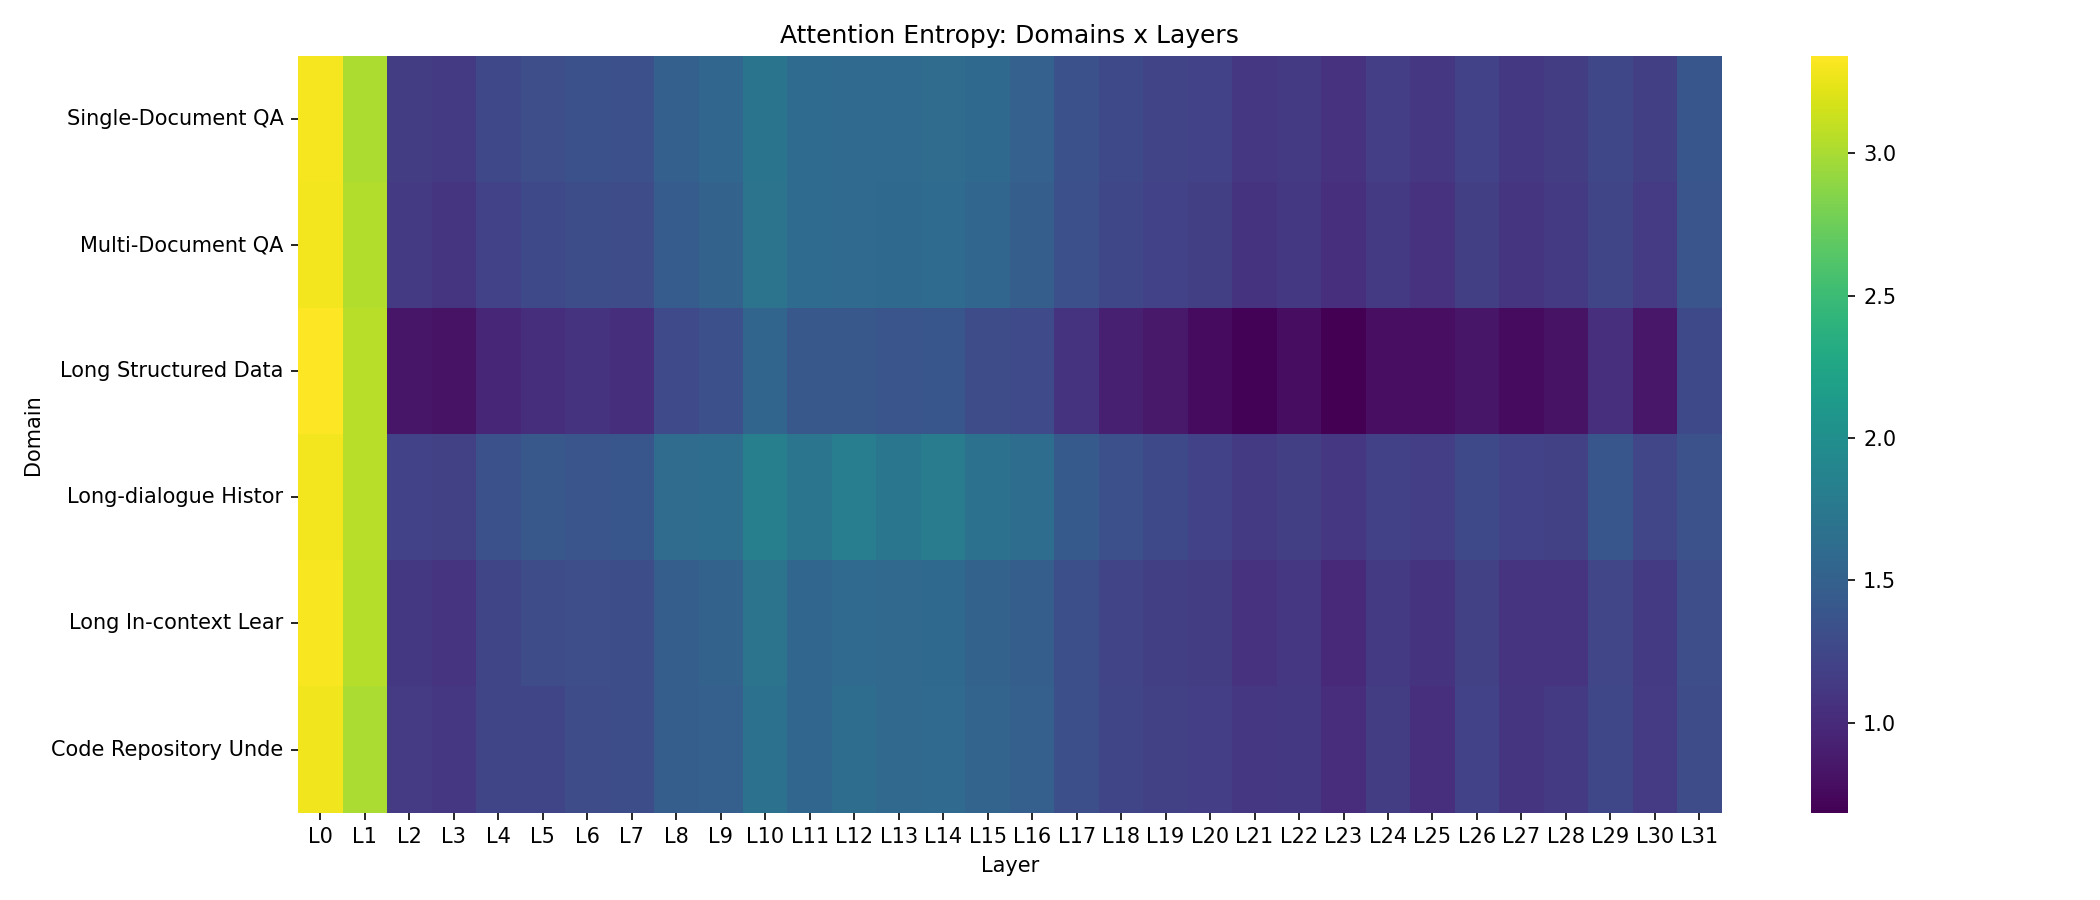
\includegraphics[width=\columnwidth]{figures/entropy_heatmap.png}
\caption{Entropy heatmap across domains and layers}
\label{fig:entropy_heatmap}
\end{figure}

\subsubsection{5.3 Entropy-Tolerance Relationship (H-M2)}

The hypothesis that high-entropy tasks tolerate eviction better was tested but yielded inconclusive results:

\begin{table}[htbp]
\centering
\resizebox{\columnwidth}{!}{%
\begin{tabular}{ll}
\toprule
Metric & Value \\
\midrule
High-entropy group mean retention & 0.067 \\
Low-entropy group mean retention & 0.000 \\
t-statistic & 1.00 \\
p-value & 0.326 \\
Cohen's d & 0.378 \\
\bottomrule
\end{tabular}
}
\end{table}

\textbf{Gate: FAIL} (p = 0.326 > 0.05 threshold)

The experiment failed due to measurement limitations rather than mechanism failure:
\begin{enumerate}
\item Baseline accuracy was 6.7\%, rendering retention ratios unreliable
\item Sample size of 30 (5 per domain) provided insufficient statistical power
\item Simple substring matching was inadequate for LongBench-v2 answer formats
\item Input truncation used to simulate eviction differs from true H2O attention-based eviction
\end{enumerate}
